\documentclass[a4paper,fleqn,usenatbib]{mnras}

\usepackage{ae, aecompl, amsmath, amssymb}
\usepackage{bm}           %%  bold math
\usepackage{cancel, mathptmx}
\usepackage{color}
\usepackage{dcolumn}  %%  Align table columns on decimal point
\usepackage{epsfig, epsf, etoolbox}
\usepackage{fancyhdr}
\usepackage{graphicx}
\usepackage[T1]{fontenc}
%\usepackage{lscape}
\usepackage{ifthen}
\usepackage{hyperref}
\usepackage{listings}
\usepackage{longtable}
\usepackage{multirow}
\usepackage{newtxtext, newtxmath}
\usepackage{pifont}% http://ctan.org/pkg/pifont
\usepackage{subfigure}
\usepackage{tabu}

\usepackage{verbatim}

\usepackage{xcolor}
%\usepackage[square, sort, comma, numbers]{natbib}
\usepackage{threeparttable}
%\usepackage[square,sort,comma,numbers]{natbib}

\usepackage{graphicx}	% Including figure files
\usepackage{tikz}
\def\checkmark{\tikz\fill[scale=0.4](0,.35) -- (.25,0) -- (1,.7) -- (.25,.15) -- cycle;} 

%%  I dont know why, but arydshln leads to pdflatex crashing (when using 'regular' hline)
%% if you load this package at the top of this list.  e.g. 
%%    tex.stackexchange.com/questions/419497/hline-doesnt-compile-arydshln-and-tabularx-incompatibility
\usepackage{arydshln}


%%%%%%%%%%%%%%%%%%%%%%%%%%%%%%%%%%%%%%%%%%%
%       define Journal abbreviations      %
%%%%%%%%%%%%%%%%%%%%%%%%%%%%%%%%%%%%%%%%%%%
\def\nat{Nat} \def\apjl{ApJ~Lett.} \def\apj{ApJ}
\def\apjs{ApJS} \def\aj{AJ} \def\mnras{MNRAS}
\def\prd{Phys.~Rev.~D} \def\prl{Phys.~Rev.~Lett.}
\def\plb{Phys.~Lett.~B} \def\jhep{JHEP}
\def\npbps{NUC.~Phys.~B~Proc.~Suppl.} \def\prep{Phys.~Rep.}
\def\pasp{PASP} \def\aap{Astron.~\&~Astrophys.} \def\araa{ARA\&A}
\def\jcap{\ref@jnl{J. Cosmology Astropart. Phys.}} 
\def\nar{New~A.R.} 

\newcommand{\preep}[1]{{\tt #1} }

%%%%%%%%%%%%%%%%%%%%%%%%%%%%%%%%%%%%%%%%%%%%%%%%%%%%%
%              define symbols                       %
%%%%%%%%%%%%%%%%%%%%%%%%%%%%%%%%%%%%%%%%%%%%%%%%%%%%%
\def \Mpc {~{\rm Mpc} }
\def \Om {\Omega_0}
\def \Omb {\Omega_{\rm b}}
\def \Omcdm {\Omega_{\rm CDM}}
\def \Omlam {\Omega_{\Lambda}}
\def \Omm {\Omega_{\rm m}}
\def \ho {H_0}
\def \qo {q_0}
\def \lo {\lambda_0}
\def \kms {{\rm ~km~s}^{-1}}
\def \kmsmpc {{\rm ~km~s}^{-1}~{\rm Mpc}^{-1}}
\def \hmpc{~\;h^{-1}~{\rm Mpc}} 
\def \hkpc{\;h^{-1}{\rm kpc}} 
\def \hmpcb{h^{-1}{\rm Mpc}}
\def \dif {{\rm d}}
\def \mlim {m_{\rm l}}
\def \bj {b_{\rm J}}
\def \mb {M_{\rm b_{\rm J}}}
\def \mg {M_{\rm g}}
\def \mi {M_{\rm i}}
\def \qso {_{\rm QSO}}
\def \lrg {_{\rm LRG}}
\def \gal {_{\rm gal}}
\def \xibar {\bar{\xi}}
\def \xis{\xi(s)}
\def \xisp{\xi(\sigma, \pi)}
\def \Xisig{\Xi(\sigma)}
\def \xir{\xi(r)}
\def \max {_{\rm max}}
\def \gsim { \lower .75ex \hbox{$\sim$} \llap{\raise .27ex \hbox{$>$}} }
\def \lsim { \lower .75ex \hbox{$\sim$} \llap{\raise .27ex \hbox{$<$}} }
\def \deg {^{\circ}}
%\def \sqdeg {\rm deg^{-2}}
\def \deltac {\delta_{\rm c}}
\def \mmin {M_{\rm min}}
\def \mbh  {M_{\rm BH}}
\def \mdh  {M_{\rm DH}}
\def \msun {M_{\odot}}
\def \z {_{\rm z}}
\def \edd {_{\rm Edd}}
\def \lin {_{\rm lin}}
\def \nonlin {_{\rm non-lin}}
\def \wrms {\langle w_{\rm z}^2\rangle^{1/2}}
\def \dc {\delta_{\rm c}}
\def \wp {w_{p}(\sigma)}
\def \PwrSp {\mathcal{P}(k)}
\def \DelSq {$\Delta^{2}(k)$}
\def \WMAP {{\it WMAP \,}}
\def \cobe {{\it COBE }}
\def \COBE {{\it COBE \;}}
\def \HST  {{\it HST \,\,}}
\def \Spitzer  {{\it Spitzer \,}}
\def \ATLAS {VST-AA$\Omega$ {\it ATLAS} }
\def \BEST   {{\tt best} }
\def \TARGET {{\tt target} }
\def \TQSO   {{\tt TARGET\_QSO}}
\def \HIZ    {{\tt TARGET\_HIZ}}
\def \FIRST  {{\tt TARGET\_FIRST}}
\def \zc {z_{\rm c}}
\def \zcz {z_{\rm c,0}}


\newcommand{\sqdeg}{deg$^{-2}$}
\newcommand{\lya}{Ly$\alpha$\ }
%\newcommand{\lya}{Ly\,$\alpha$\ }
\newcommand{\lyaf}{Ly\,$\alpha$\ forest}
%\newcommand{\eg}{e.g.~}
%\newcommand{\etal}{et~al.~}
\newcommand{\cii}{C\,{\sc ii}\ }
\newcommand{\ciii}{C\,{\sc iii}]\ }
\newcommand{\civ}{C\,{\sc iv}}
\newcommand{\siiv}{Si\,{\sc iv}\ }
\newcommand{\mgii}{Mg\,{\sc ii}\ }
\newcommand{\feii}{Fe\,{\sc ii}\ }
\newcommand{\feiii}{Fe\,{\sc iii}\ }
\newcommand{\caii}{Ca\,{\sc ii}\ }
\newcommand{\halpha}{H\,$\alpha$\ }
\newcommand{\hbeta}{H\,$\beta$\ }
\newcommand{\oi}{[O\,{\sc i}]\ }
\newcommand{\oii}{[O\,{\sc ii}]\ }
\newcommand{\oiii}{[O\,{\sc iii}]\ }
\newcommand{\heii}{[He\,{\sc ii}]\ }
\newcommand{\nii}{N\,{\sc ii}\ }
\newcommand{\nv}{N\,{\sc v}\ }

%% From:: /cos_pc19a_npr/LaTeX/proposals/JWST/JWST_ERS/Proposal/lines.tex
%%  
\newcommand{\imw}{$i$--$W3$}
\newcommand{\imwf}{$i$--$W4$}
\newcommand{\rmwf}{$r$--$W4$}
\newcommand{\imwt}{$i$--$W2$}
\newcommand{\wtmwf}{$W3$--$W4$}
%\newcommand{\kms}{km s$^{-1}$}
\newcommand{\cmN}{cm$^{-2}$}
\newcommand{\cmn}{cm$^{-3}$}
%\newcommand{\msun}{M$_{\odot}$}
\newcommand{\lsun}{L$_{\odot}$}
\newcommand{\lam}{$\lambda$}
\newcommand{\mum}{$\mu$m}
\newcommand{\ebv}{$E(B$$-$$V)$}
%\newcommand{\heii}{\mbox{He\,{\sc ii}}}
\newcommand{\cv}{\mbox{C\,{\sc v}}}
%\newcommand{\civ}{\mbox{C\,{\sc iv}}}
%\newcommand{\ciii}{\mbox{C\,{\sc iii}}}
%\newcommand{\cii}{\mbox{C\,{\sc ii}}}
%\newcommand{\nv}{\mbox{N\,{\sc v}}}
\newcommand{\niv}{\mbox{N\,{\sc iv}}}
\newcommand{\niii}{\mbox{N\,{\sc iii}}}
%\newcommand{\oi}{\mbox{O\,{\sc i}}}
%\newcommand{\oii}{\mbox{O\,{\sc ii}}}
%\newcommand{\oiii}{\mbox{[O\,{\sc iii}]}}
\newcommand{\oiv}{\mbox{O\,{\sc iv}}}
\newcommand{\ov}{\mbox{O\,{\sc v}}}
\newcommand{\ovi}{\mbox{O\,{\sc vi}}}
\newcommand{\ovii}{\mbox{O\,{\sc vii}}}

%\newcommand{\feii}{\mbox{Fe\,{\sc ii}}}
%\newcommand{\feiii}{\mbox{Fe\,{\sc iii}}}
%\newcommand{\mgii}{\mbox{Mg\,{\sc ii}}}
\newcommand{\neii}{[Ne\,{\sc ii}]\ }
\newcommand{\neiii}{[Ne\,{\sc ii}]\ }
\newcommand{\nev}{Ne\,{\sc v}\ }
\newcommand{\nevi}{[Ne\,{\sc vi}]\ }
\newcommand{\neviii}{\mbox{Ne\,{\sc viii}}}
\newcommand{\aliii}{\mbox{Al\,{\sc iii}}}
\newcommand{\siii}{\mbox{Si\,{\sc ii}}}
\newcommand{\siiii}{\mbox{Si\,{\sc iii}}}
%\newcommand{\siiv}{\mbox{Si\,{\sc iv}}}
%\newcommand{\lya}{\mbox{Ly$\alpha$}}
%\newcommand{\lyb}{\mbox{Ly$\beta$}}
\newcommand{\hi}{\mbox{H\,{\sc i}}}
\newcommand{\snine}{\mbox{[S\,{\sc ix}]}}
\newcommand{\sivi}{\mbox{[Si\,{\sc vi}]}}
\newcommand{\sivii}{\mbox[{Si\,{\sc vii}]}}
\newcommand{\siix}{\mbox{[Si\,{\sc ix}]}}
\newcommand{\six}{\mbox{[Si\,{\sc x}]}}
\newcommand{\sixi}{\mbox{[Si\,{\sc xi}]}}
\newcommand{\caviii}{\mbox{[Ca\,{\sc viii}]}}
\newcommand{\arii}{\mbox{[Ar\,{\sc ii}]}}

%%[Ar II] 6.97
%% [S IX] 1.252 μm 328 
% [Si X] 1.430 μm 351 
% [Si XI] 1.932 μm 401 
% [Si VI] 1.962 μm 167 
% [Ca VIII] 2.321 μm 128 
% [Si VII] 2.483 μm 205 
% [Si IX] 3.935 μm 303
% [Ar II] 6.97


%\snine\ at 1.252$\mu$m, \six\ at 1.430$\mu$m, \sixi\ at 1.932$\mu$m, \sivi\ at
%1.962$\mu$m, \caviii\ at 2.321$\mu$m, \sivi\ at 2.483$\mu$m \siix\ at
%3.935$\mu$m and \arii\ at 6.97$\mu$m. 
%%
%% such as [Ne ii]12.8 μm, [Ne v]14.3 μm, [Ne iii]15.5 μm, [S iii]18.7 μm and 33.48 μm, [O iv]25.89 μm and [Si ii]34.8 μm (e.g
%%
%% MIR emission lines like [NeII] and [NeV] are ..
%%
%% Also,  arXiv:astro-ph/0003457v1 
%% [NeV] 14.32um & 24.32um and [NeVI] 7.65um imply an A(V)>160 towards the NLR...
%% [NeIII]15.56um/[NeII]12.81um
%%
%% [Ne V] 14.3, 24.2 μm 97.
%% [Ne II] 12.8 μm
%% [OIV] 26μm
%%


%%%%%%%%%%%%%%%%%%%%%%%%%%%%%%%%%%%%%%%%%%%%%%%%%%%%%
%              define Listings                       %
%%%%%%%%%%%%%%%%%%%%%%%%%%%%%%%%%%%%%%%%%%%%%%%%%%%%%
\definecolor{dkgreen}{rgb}{0,0.6,0}
\definecolor{gray}{rgb}{0.5,0.5,0.5}
\definecolor{mauve}{rgb}{0.58,0,0.82}

\lstset{frame=tb,
  language=Python,
  aboveskip=3mm,
  belowskip=3mm,
  showstringspaces=false,
  columns=flexible,
  basicstyle={\small\ttfamily},
  numbers=none,
  numberstyle=\tiny\color{gray},
  keywordstyle=\color{blue},
  commentstyle=\color{dkgreen},
  stringstyle=\color{mauve},
  breaklines=true,
  breakatwhitespace=true,
  tabsize=3
}


\title[High-redshift CLQs]{The first high-redshift Changing Look Quasars}

\author[Bercow]
{The RH John~S.~Bercow, MP, {\it et al.} 
%Nicholas~P.~Ross$^{1}$\thanks{E-mail: npross@roe.ac.uk},    
%K. E. Saavik Ford$^{2,3,4}$,  Matthew Graham$^{5}$,  Barry McKernan$^{2,3,4}$,  
%\newauthor Daniel Stern$^{6}$, 
\\
% List of institutions
$^{1}$Speaker's Chair, The House of Commons, London, SW1A 0AA \\
%$^{1}$Institute for Astronomy, University of Edinburgh, Royal Observatory, Blackford Hill, Edinburgh EH9 3HJ, United Kingdom \\
%$^{2}$Department of Science, BMCC, City University of New York, New York, NY 10007, USA \\
%$^{3}$Department of Astrophysics, Rose Center for Earth and Space, American Museum of Natural History, Central Park West at 79th Street, NY 10024, USA \\
%$^{4}$Graduate Center, City University of New York, 365 5th Avenue, New York, NY 10016, USA\\
%$^{5}$Cahill Center for Astronomy and Astrophysics, California Institute of Technology, Mail Code 249/17, 1200 E California Blvd, Pasadena CA 91125, USA\\
%$^{6}$Jet Propulsion Laboratory, California Institute of Technology, 4800 Oak Grove Drive, Mail Stop 169-221, Pasadena, CA 91109, USA \\
}


\date{Accepted XXX. Received YYY; in original form ZZZ}
\pubyear{2018}

\hypersetup{draft}
\begin{document}
\label{firstpage}
\pagerange{\pageref{firstpage}--\pageref{lastpage}}
\maketitle

\begin{abstract}
We report on three redshift $z>2$ quasars with dramatic changes in
their \civ\ emission lines, the first `Changing-Look'' quasars at high
redshift.  This is also the first time the changing-look behaviour has
been seen in a high-ionization emissions line.
%%
SDSS J1205+3422, J1638+2827 and J2228+2201 show interesting behaviour
in their observed optical light curves, and subsequent spectroscopy
shows significant changes in the \civ\ broad emission line, with both
line collapse and emergence being displayed in rest-frame timescales
of $\sim$240-1640 days.
%%
Where observed, the profile of the Ly$\alpha$/\nv emission complex
also changes, and there is tentative evidence for changes in the \mgii
line.
%%
Although line measurements from the three quasars show large changes
in the \civ\ line flux-line width plane, the quasars are not seen to
be outliers when considered against the full $z>2$ quasar population
in terms of (rest) Equivalent Width and FWHM properties.
%%
We put these observations in context with recent ``state-change''
models, but note that even in their `low-state', the \civ\ CLQs are
above $\sim10\%$ in Eddington luminosity.
\end{abstract}



% Select between one and six entries from the list of approved keywords.
% Don't make up new ones.
\begin{keywords}
accretion, accretion discs -- surveys -- quasars: general -- quasars: individual: J1100-0053 
\end{keywords}



%%%%%%%%%%%%%%%%%%%%%%%%%%%%%%%%%%%%%%%%%%%%%%%%%%%%%%%%%%%%%%%%%%%%%%%%%%%%%%%%%
%%%%%%%%%%%%%%%%%%%%%%%%%%%%%%%%%%%%%%%%%%%%%%%%%%%%%%%%%%%%%%%%%%%%%%%%%%%%%%%%%
%%
%%
%%   SECTION 1  SECTION 1  SECTION 1  SECTION 1  SECTION 1  SECTION 1  
%%   SECTION 1  SECTION 1  SECTION 1  SECTION 1  SECTION 1  SECTION 1  
%%   SECTION 1  SECTION 1  SECTION 1  SECTION 1  SECTION 1  SECTION 1  
%%
%%
%%%%%%%%%%%%%%%%%%%%%%%%%%%%%%%%%%%%%%%%%%%%%%%%%%%%%%%%%%%%%%%%%%%%%%%%%%%%%%%%%%
%%%%%%%%%%%%%%%%%%%%%%%%%%%%%%%%%%%%%%%%%%%%%%%%%%%%%%%%%%%%%%%%%%%%%%%%%%%%%%%%%%
\section{Introduction}
Luminous AGN, i.e. quasars, are now seen to significantly vary their
energy output on timescales of weeks to months.  This observation, and
the subsequent mismatch in the expected ``viscous'' timescale, which
for a $\approx$10$^{7}$ M$_{\odot}$ is $\sim$hundreds of years, was
noted over 30 years ago \citep[e.g.][]{Alloin1985}. However, with new
photometric light-curve and repeat spectroscopic data, the desire for
a deeper understanding of AGN accretion disk physics has been recently
re-invigorated the field \citep[e.g.][]{Lawrence2018, Antonucci2018}.

The optical continuum variability of quasars has been recognized since
their first optical identification
\citep[e.g.,][]{MatthewsSandage1963, MacLeod2012}.  Dramatic
changes in the broad emission lines (BELs) of quasars has only
recently been identified \citep[e.g., ][]{LaMassa2015}.  Samples of over
100 ``Changing Look'' quasars (CLQs) or ``Changing State'' quasars
(CSQs) have now been assembled \citep[e.g.][]{MacLeod2019,Graham2019}.
The community uses both these terms as a cover for the underlying
physics. For sake of argument, ``Changing Look'' quasars can
potentially be thought of as the extension to the BELs of quasar
continuum variability \citep[e.g., ][]{MacLeod2012} whereas the
``Changing State'' quasars (CSQs) have a `state-transition' similar to
that in Galactic X-ray binaries \citep[][]{NodaDone2018,
Ruan2019}. In this paper, we use the term `Changing Look', as we are
currently agnostic, and somewhat ignorant, to the underlying physical
processes.

These CLQs have primarily been defined according to the
(recombination) Balmer emission line properties with particular
attention paid to the H$\beta$ emission line, usually observed from
optical spectroscopy.  As such, current CLQ studies have been at
redshifts $z<1$.

While there have been a slew of studies on triply ionized carbon, i.e
\civ, these have tended to focus on broad absorption line quasars
\citep[BAL QSOs; see Table 1][]{Hemler2019} or the Baldwin Effect
\citep[BEff; ][]{Baldwin1977, Bian2012, Jensen2016,
Hamann2017}\footnote{As noted in \citet{Rakic2017}, two different
types of Baldwin effect are present in the literature: the {\it
global} (or {\it ensemble}) Baldwin Effect, which is an
anti-correlation between the EW of the emission line and the
underlying continuum luminosity of {\it single-epoch} observations of
a {\it large number} of AGN and second, the {\it intrinsic} Baldwin
effect, the same anti-correlation but in an {\it individual, variable}
AGN \citep{PoggePeterson1992}.}.  Dramatic changes in the
collisionally excited broad {\it emission} line (BEL) of \civ\ (and
indeed \ciii) have not to this point been seen.

Here, we report on three quasars  
which show dramatic changes in their \civ\ and \ciii broad emission
line properties as well as in the underlying continuum. We claim these
are the first examples of ``Changing Look Quasars'' at high ($z>1$)
redshift. Moreover, these are the first cases for substantial changes
of ions with high ionization potentials (I.P.'s $>$2 Rydberg), thus
linking the ionizing photons to the energetic inner accretion disk,
potentially by inverse Compton scattering of lower energy photons to
higher energies.  Furthermore, the measured rest-wavelengths of
emission lines in quasar spectra, are known to vary from their nominal
laboratory wavelengths especially for the high-ionization broad lines \citep[e.g.][]{VandenBerk2001}.

In this paper we use the wavelengths of 1548.202 and 1550.774~\AA\ for
the \civ\ doublet \citep{Kramida2018}. The ground state of carbon is
1$s^2$ 2$s^2$ 2$p^2$.  Using the
\href{https://physics.nist.gov/PhysRefData/ASD/ionEnergy.html}{NIST
Atomic Spectra Database Ionization Energies Form} for ionisation
energies, we note 11.3 eV is the energy required for C~I to dislodge
one electron and become singly-ionised C~II; 24.4 eV is then the
(`additional') energy needed for singly-ionised C~II to dislodge an
additional electron, and become doubly-ionised C~III, and 47.89 eV
(3.519 Ry) is required for doubly-ionised C~III become triply-ionised
\civ.  64.49 eV (4.74 Ry) is the energy needed to ionize \civ\
itself. The 1548.202 and 1550.774 \AA\ emission doublet is created by
the 2$p$ $^{2}P_{0}$ $-$ 2$s$ $^{2}S$ transition with energies 64,484
cm$^{-1}$ and 64,591 cm$^{-1}$ \citep[e.g.][]{Moore1993}.
 
%%       B a c k g r o u n d     L i t e r a t u r e    
\civ\ variability has been long studied, e.g., \citet[][]{Baldwin1977,
Gaskell1982, Gregory1982, Wilkes1986, Espey1989, Espey1990Erratum,
ZhengSulentic1990, Corbin1990, Corbin1991, Weymann1991,
Dimitrijevic1992, TytlerFan1992, Wills1993, Brotherton1994, Osmer1994,
Laor1995, McIntosh1999, Nazarova2003}.  

\citet{Wilhite2006} examine
the variability of a C~\textsc{iv} sample of 105 quasars observed at
multiple epochs by the SDSS.  They find a strong correlation between
the change in the C~\textsc{iv} line flux and the change in the line
width, but no correlations between the change in flux and changes in
line center and skewness.  These authors find that the relation
between line flux change and line width change is consistent with a
model in which a broad line base varies with greater amplitude than
the line core. The C~\textsc{iv} lines in these high-luminosity
quasars appear to be less responsive to continuum variations than
those in lower luminosity AGN.  \citet{Wilhite2006} find no evidence
for variability of the well known blueshift of the C~\textsc{iv} line
with respect to the low-ionization Mg~\textsc{ii}$\lambda$2798 line in
the highest flux objects.

\citet{Richards2011} explored the BEL region in over 30,000 $z > 1.54$ SDSS
quasars, concentrating on the properties of the \civ\ emission
line. We consider two well-known effects involving the \civ\ emission
line: the anti-correlation between the \civ\ EQW and luminosity (i.e.,
the BEff) and the blueshifting of the peak of \civ\ emission with
respect to the systemic redshift. These authors conclude that these
two \civ\ parameters (EQW and blueshift) are capturing an important
trade-off between ``disk'' and ``wind'' components in the disk-wind
model of accretion disks \citep[e.g.,][]{Murray1995, Elvis2000,
Proga2000}.  with one dominating over the other depending on the shape
of the SED \citep[][strong \civ\ EQW indicates a more ionizing SED and
large \civ\ blueshift indicating a less ionizing SED]{Leighly2004b}.

The Sloan Digital Sky Survey Reverberation Mapping Project
\cite[(SDSS-RM)][]{Shen2015} has a monitored $\sim$350 quasars with
\civ. Noting the biases associated with \civ Emission Line Properties
\citep[e.g. increasing systematic offsets with decreasing
signal-to-noise][]{Denney2016}, \citet{Grier2019} report report
significant time delays between the continuum and the CIV 1549
emission line in 52 quasars, and investigate the \civ
radius-luminosity relationship.

\civ\ is also known to exhibit significant displacements to the
blue and these `blueshifts' almost certainly signal the presence of
strong outflows. As a consequence, single-epoch virial black hole (BH)
mass estimates derived from \civ\ velocity widths are known to be
systematically biased compared to masses from the hydrogen Balmer
lines. \citet{Coatman2017} use a large sample of 230 high-luminosity
($L$Bol = 1045.5-1048 erg s-1), redshift $1.5 < z < 4.0$ quasars with
both \civ\ and Balmer line spectra, we have quantified the bias in \civ
BH masses as a function of the \civ\ blueshift. \civ\ BH masses are
shown to be a factor of 5 larger than the corresponding Balmer-line
masses at C IV blueshifts of 3000 km s$^{-1}1$ and are overestimated
by almost an order of magnitude at the most extreme blueshifts,
$\gtrsim$5000 km s$^{-1}$.

\citet{Sun2018} use the multi-epoch spectra of 362 quasars from the
Sloan Digital Sky Survey Reverberation Mapping project to investigate
the dependence of the blueshift of \civ\ relative to \mgii on quasar
properties. We confirm that high-blueshift sources tend to have low
\civ\ equivalent widths (EWs), and that the low-EW sources span a range
of blueshift. Other high-ionization lines, such as He II, also show
similar blueshift properties. The ratio of the line width (measured as
both the full width at half maximum and the velocity dispersion) of
\civ\ to that of \mgii increases with blueshift. Quasar variability
enhances the connection between the \civ\ blueshift and quasar
properties (e.g., EW). The variability of the \mgii line center (i.e.,
the wavelength that bisects the cumulative line flux) increases with
blueshift. In contrast, the C IV line center shows weaker variability
at the extreme blueshifts. Quasars with the high-blueshift \civ\ lines
tend to have less variable continuum emission, when controlling for
EW, luminosity, and redshift. Our results support the scenario that
high-blueshift sources tend to have large Eddington ratios.
Therefore, according to this study, the \civ\ or \heii\ EW is not an
accurate indicator of the Eddington ratio or quasar SED.
%%
Recent investigations also include \citet{Meyer2019} and \citet{Doan2019}. 

The purpose of this paper is, for the first time, to access and 
report on the Changing-Look quasar phenomenon at high, 
$z>2$ redshift. By doing so, we move from the low-ionization 
energy Balmer emission line series to the high-ionization emission 
lines, in particular \civ\ $\lambda$1549. 

This paper is organised as follows. In Section 2, we describe our
sample selection, catalogs and observational data sets.  In Section 3,
we present the high-$z$ quasars and report the line properties for the
quasars at the observed epochs.  We give a very brief theoretical
discussion in Section 4. We present our Conclusions in Section 5.  We
report all magnitudes on the AB zero-point system \citep{Oke_Gunn1983,
Fukugita1996} unless otherwise stated explicitly. For the WISE bands,
$m_{\rm AB} = m_{\rm Vega} + m$ where $m = (2.699, 3.339)$ for WISE W1
at 3.4$\mu$m and WISE W2 at 4.6$\mu$m, respectively
\citep{Cutri2011}. We choose the cosmological parameters
$\Omega_{\Lambda} = 0.7$, $\Omega_{\rm M} = 0.3$, and $h = 0.7$ in
order to be consistent with \citet{Shen2011}.


%%%%%%%%%%%%%%%%%%%%%%%%%%%%%%%%%%%%%%%%%%%%%%%%%%%%%%%%%%%%%%%%%%%%%%%%%%%%%
%%%%%%%%%%%%%%%%%%%%%%%%%%%%%%%%%%%%%%%%%%%%%%%%%%%%%%%%%%%%%%%%%%%%%%%%%%%%%
%%
%%   SECTION 2   SECTION 2   SECTION 2   SECTION 2   SECTION 2   SECTION 2  
%%   SECTION 2   SECTION 2   SECTION 2   SECTION 2   SECTION 2   SECTION 2  
%%   SECTION 2   SECTION 2   SECTION 2   SECTION 2   SECTION 2   SECTION 2  
%%
%%%%%%%%%%%%%%%%%%%%%%%%%%%%%%%%%%%%%%%%%%%%%%%%%%%%%%%%%%%%%%%%%%%%%%%%%%%%%
%%%%%%%%%%%%%%%%%%%%%%%%%%%%%%%%%%%%%%%%%%%%%%%%%%%%%%%%%%%%%%%%%%%%%%%%%%%%%
\begin{table*}
  \centering
  \begin{tabular}{r  r  r r r   r r r r}
    \hline 
    \hline 
    Object                         & \multirow{3}{*}{Redshift} & \multirow{3}{*}{$g$-band mag}      & \multirow{3}{*}{MJD} & \multirow{3}{*}{Date}  & \multirow{3}{*}{Instrument}  & Exposure      & SDSS                        & \multirow{3}{*}{Notes} \\
    R.A. / deg                   &                                         &                                                          &                                 &                                   &                                               &  Time           & Spectrum                 & \\
    Decl. / deg                 &                                         &                                                          &                                &                                     &                                              &  / seconds    & Plate-FiberID  & \\
    \hline 
                                   &                                          &                        &             &                            &                    &                             &                              & \\
    J120544.7+342252.4  & 2.068$\pm$0.0003          &   18.27             & 53498  &  2005-May-08   & SDSS             & tbd                          & 2089-427             & \\
    181.436164          & 2.071                               & {\bf 17.99?}   & 58538  &  2019-Feb-24    & DBSP            &  2$\times$900    &                               &  Conditions? \\
    +34.381229           &                                        &                          & 58693  &  2019-Jul-29     & DBSP            &  2$\times$1200   &                              &   \\
                                   &                                        &                          &              &                          &                   &                                &                              & \\
    J163852.9+282707.7   & 2.185$\pm$0.0004       &   19.77               & 54553 & 2008-Mar-28     & SDSS             & tbd                          &  2948-614              & \\
    249.720558	             &  2.186$\pm$0.0007      &                           & 55832  & 2011-Sep-28     & BOSS            &   3603                  &  5201-178            & \\
    +28.452159             &  2.182                           &                           & 58583 & 2019-Apr-10      & LRIS              &  2$\times$900    &                              & \\
                                   &                                      &                          &              &                           &                   &                              &                                & \\
    J222818.7+220102.9   & 2.217$\pm$0.0021      & 19.97                 & 56189 & 2012-Sep-19      & BOSS             &  2702                 &   6118-720          & \\
    337.078194             & 2.222$\pm$0.0004      &                          & 56960 & 2014-Oct-30      & BOSS             & tbd                         &   7582-790          & QSO1-REOBS \\ 
    +22.017478            &                                      &                          & 58693 & 2019-Jul-29        & DBSP              & 2$\times$1200  &                           &    \\
                                   &                                     &                           &            &                             &                   &                              &                            & \\
    \hline \hline   
  \end{tabular}
  \caption{
    Details of our spectroscopic observations. 
    Exposure times are from the {\tt plate.fits} file.  SDSS, BOSS and
    eBOSS spectra have $\mathcal{R}\sim$2,000.  DBSP is the
    $\mathcal{R}\sim$1,000-10,000 resolution Double Spectrograph for the
    Palomar 200-inch telescope.  LRIS is the Low Resolution Imaging
    Spectrometer on the Keck I 10m telescope.} 
  \label{tab:obs_notes}
\end{table*}
\section{Data}
%% \subsection{Selection/Identification}
{\bf MJG to write a few notes on how the CIV CLQs were identified} 
lorem ipsum dolor sit amet, consectetur adipiscing elit. Aliquam
porta sodales est, vel cursus risus porta non. Vivamus vel pretium
velit. Sed fringilla suscipit felis, nec iaculis lacus convallis
ac. Fusce pellentesque condimentum dolor, quis vehicula tortor
hendrerit sed. Class aptent taciti sociosqu ad litora torquent per
conubia nostra, per inceptos himenaeos. Etiam interdum tristique diam
eu blandit. Donec in lacinia libero.

SDSS J120544.7+342252.4  (hereafter J1205+3422), 
SDSS J163852.93+282707.7 (hereafter J1638+2827) and
SDSS J222818.76+220102.9 (hereafter J2228+2201). 
Sed elit massa, eleifend non sodales a, commodo ut felis. Sed id
pretium felis. Vestibulum et turpis vitae quam aliquam convallis. Sed
id ligula eu nulla ultrices tempus. Phasellus mattis erat quis metus
dignissim malesuada. Nulla tincidunt quam volutpat nibh facilisis
euismod. Cras vel auctor neque. Nam quis diam risus.




\begin{figure*}
  \centering
  %% trim=l b r t
  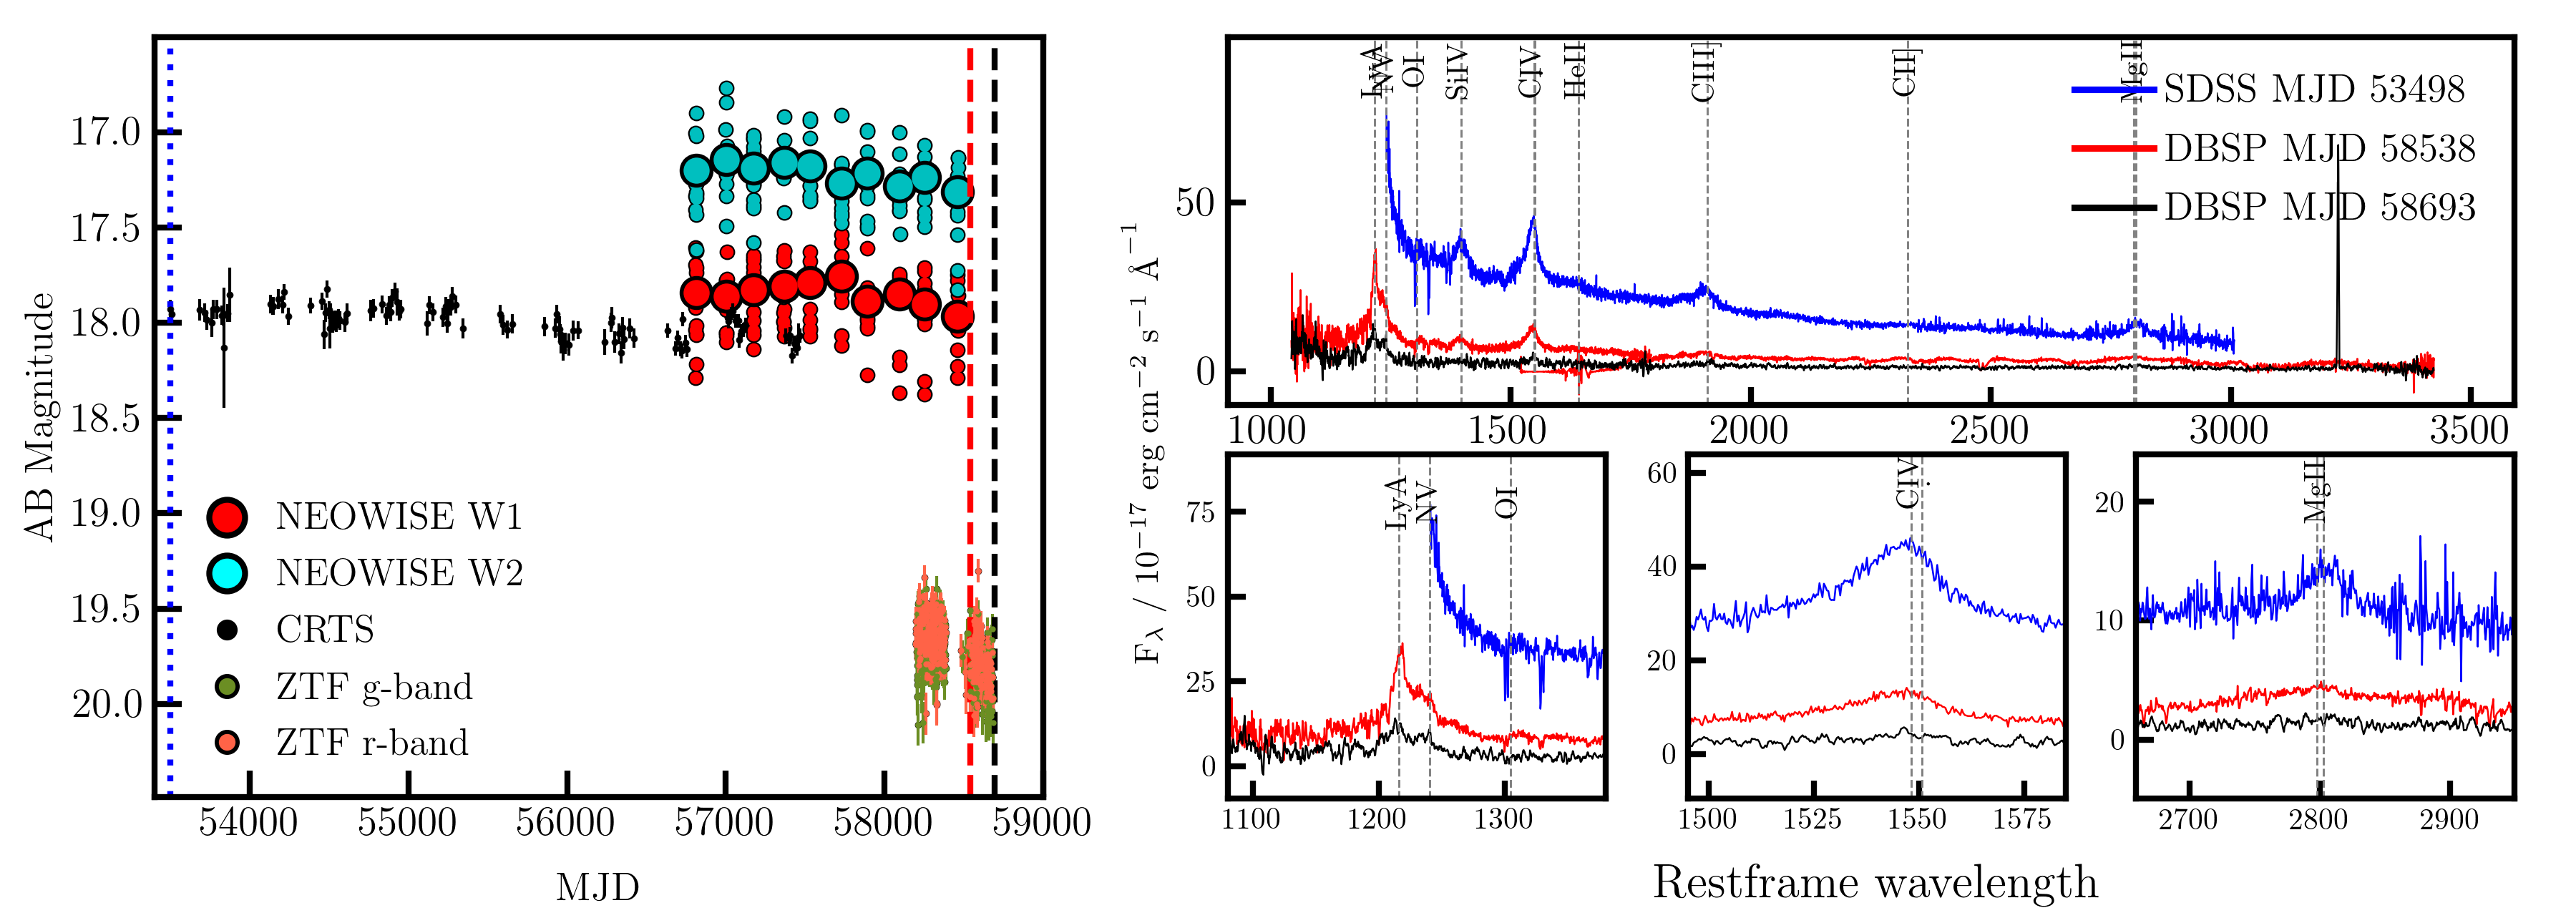
\includegraphics[width=16.7cm, trim=0.0cm 0.05cm 0.2cm 0.1cm, clip]
  {figures/J1205+3422_landscape_20190920.png}
  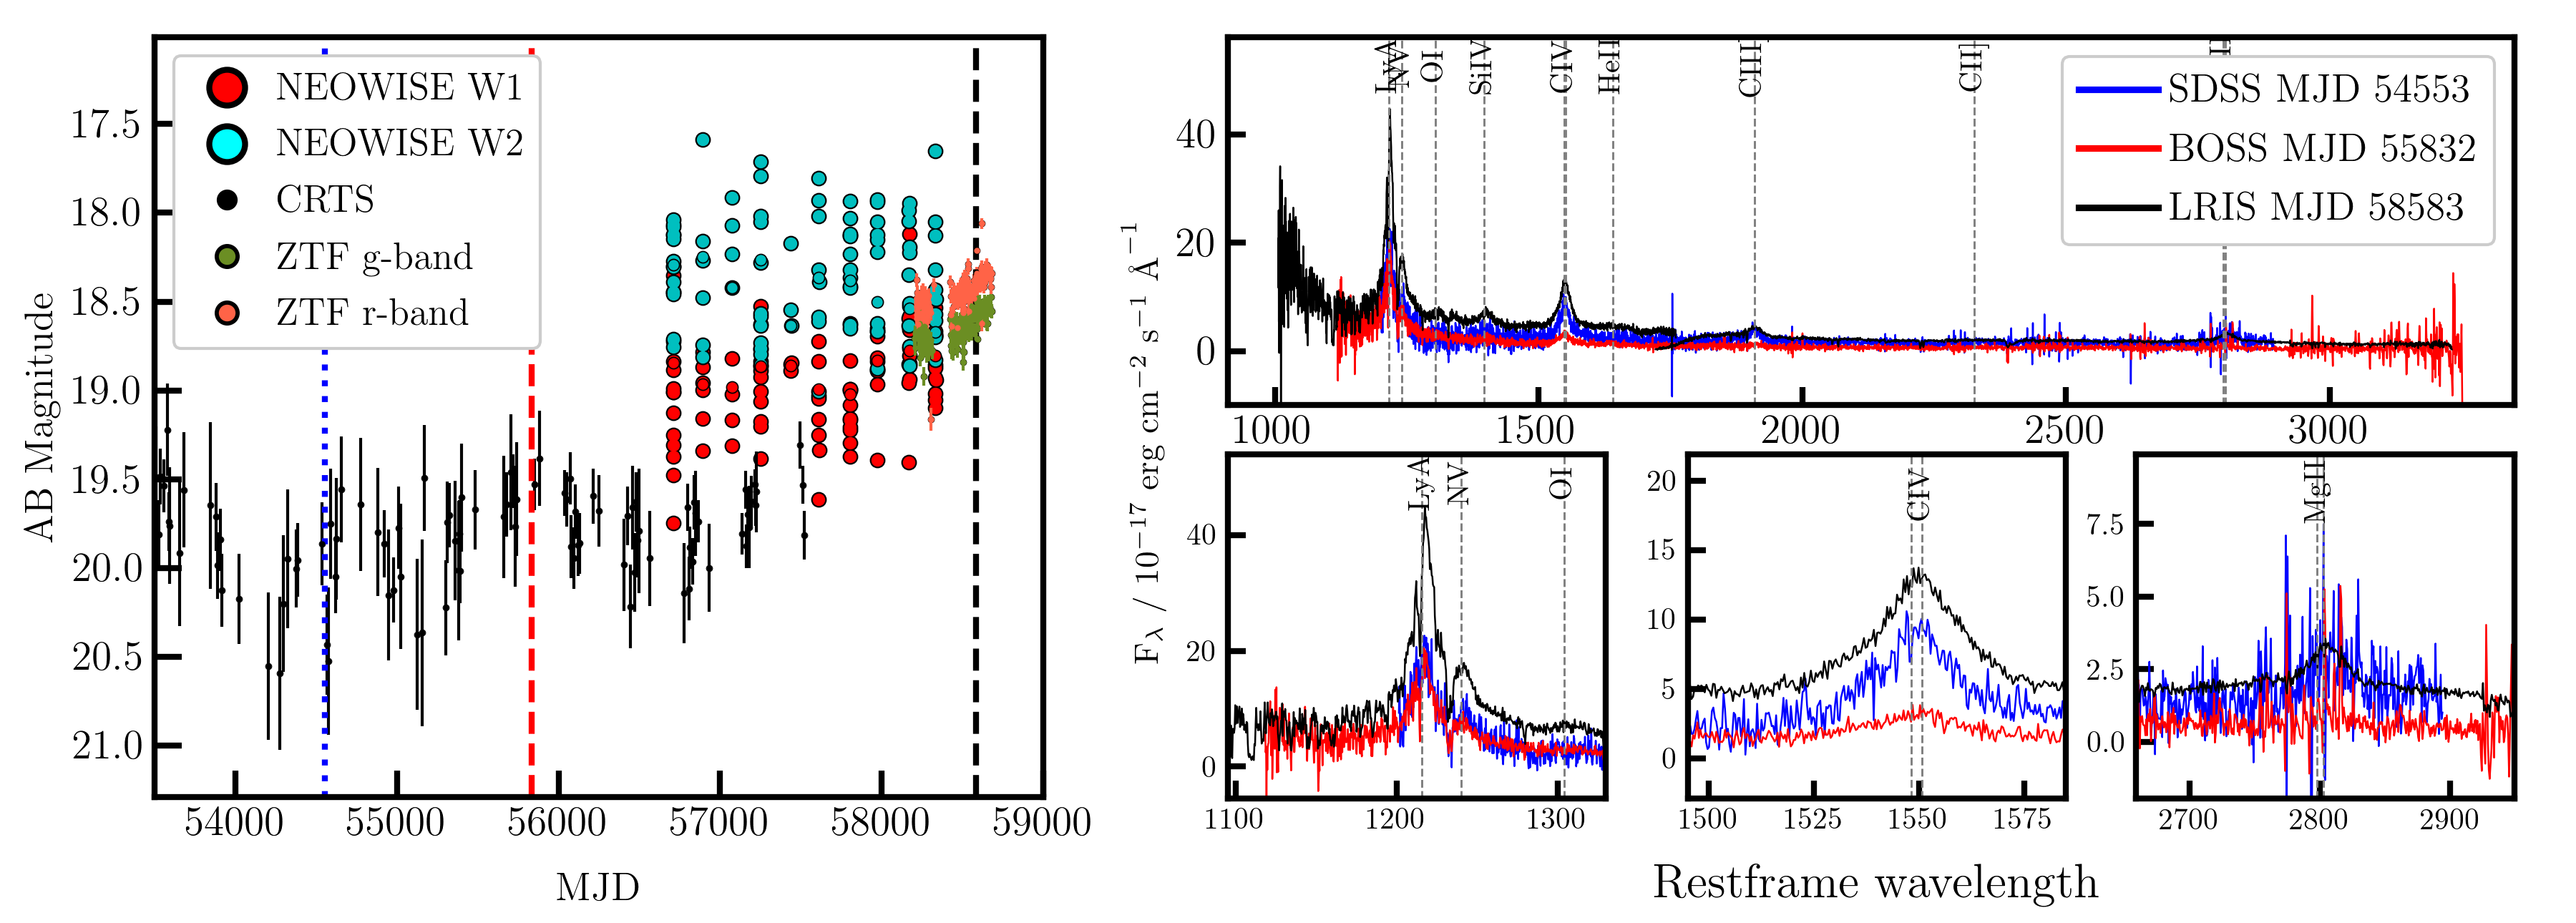
\includegraphics[width=16.7cm, trim=0.0cm 0.05cm 0.2cm 0.1cm, clip]
  {figures/J1638+2827_landscape_20190920.png}
  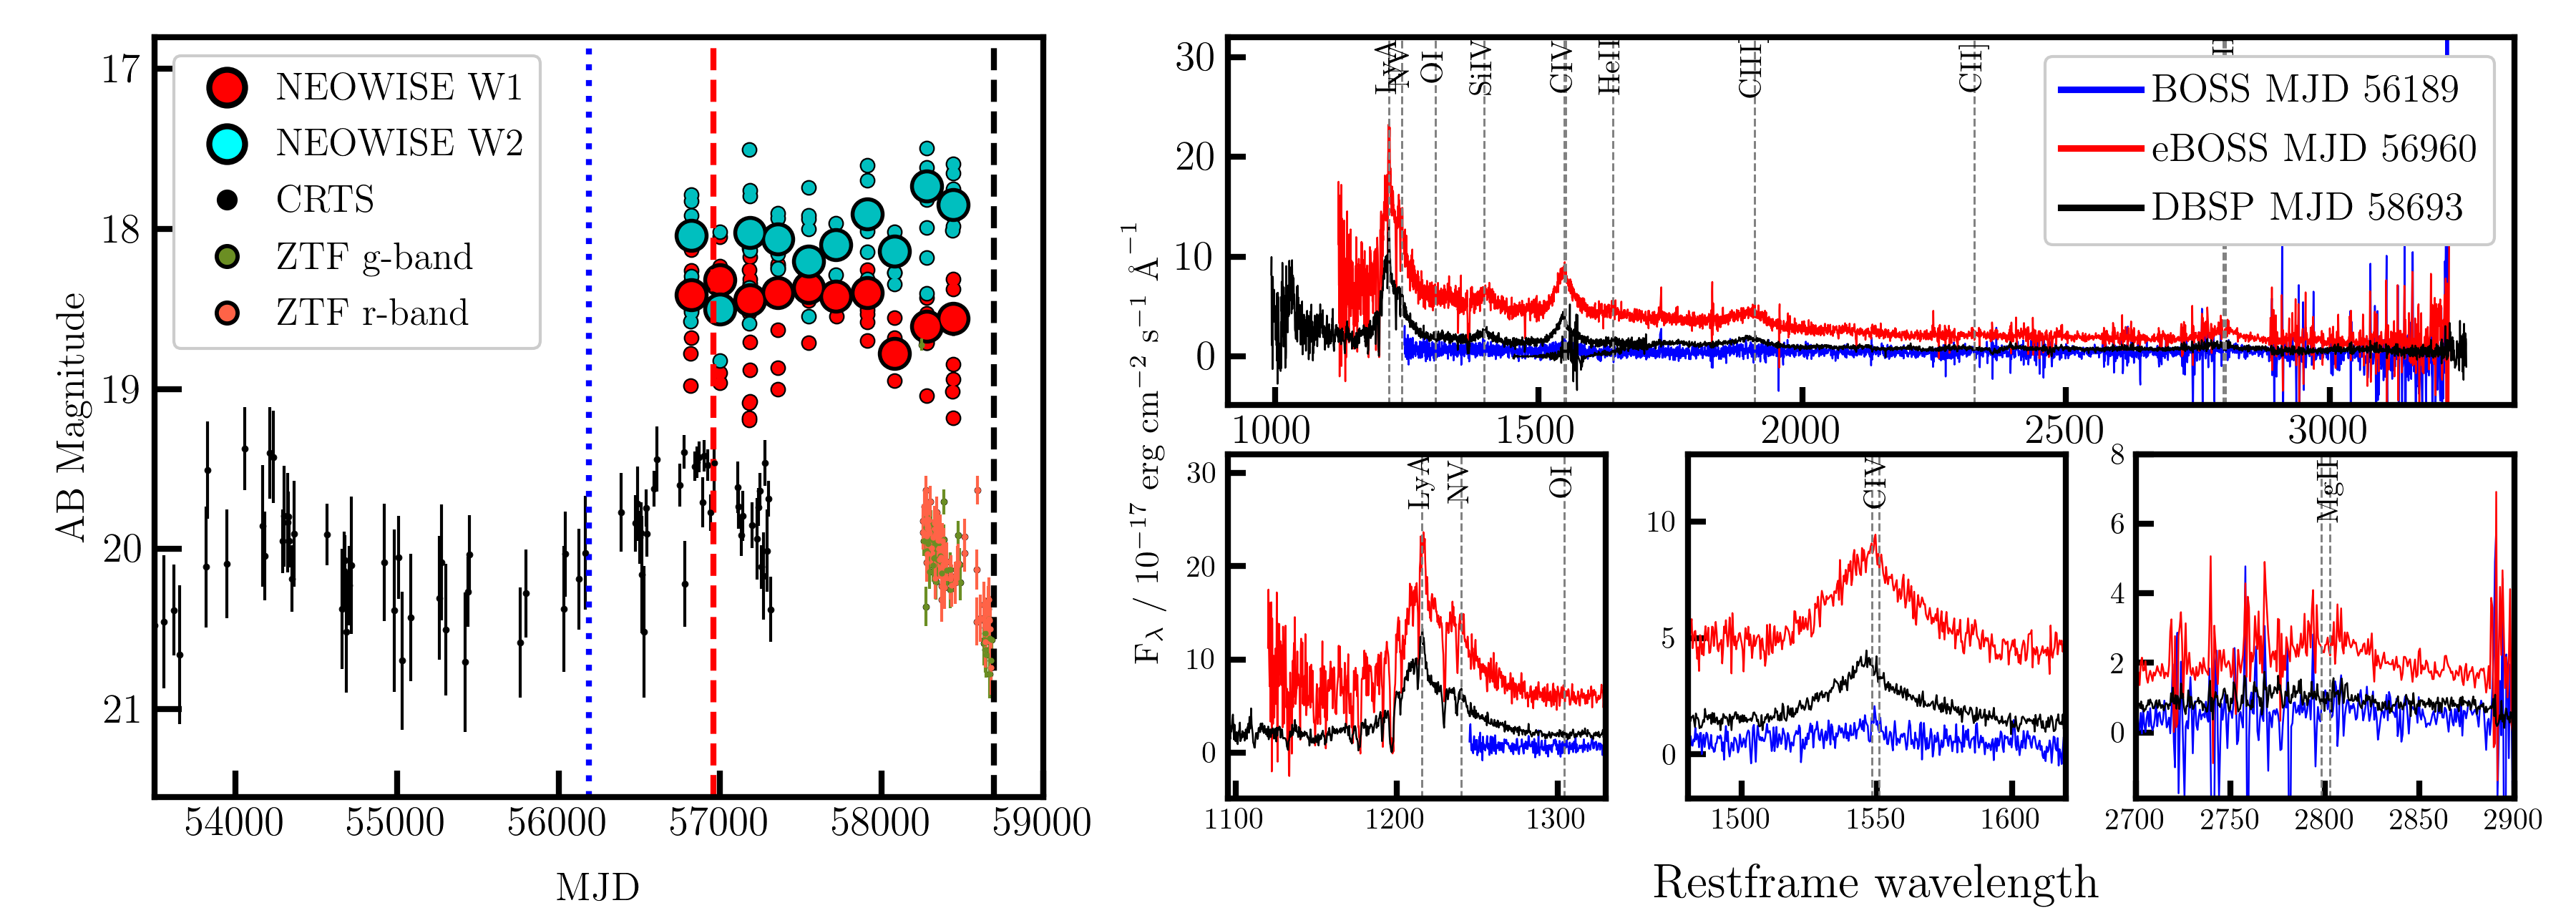
\includegraphics[width=16.7cm, trim=0.0cm 0.0cm  0.2cm 0.1cm, clip]
  {figures/J2228+2201_landscape_20190920.png}
  \vspace{-12pt}
  \caption[]{The threes high-$z$ CLQ quasars; 
    SDSS J1205+3422 (top), 
    SDSS J1638+2827 (middle), 
    SDSS J2228+2201 (bottom). 
The light curve data is present in the panels on the left hand side, with the 
spectral epoch observational timings given by the vertical lines. 
The spectra are on the right hand side, with zoom-in's on the Ly$\alpha$-\nv 
complex, the \civ\ line and the \mgii line. 
  }
  \label{fig:civ_clqs}
\end{figure*}
\subsection{Spectra}
An overview of our spectroscopic observations is given in
Table~\ref{tab:obs_notes}.  The spectra are from the SDSS
\citep{Stoughton2002, DR7, Schneider2010}, the SDSS-III Baryon
Oscillation Spectroscopic Survey \citep[BOSS][]{Eisenstein2011,
Dawson2013, Smee2013, Alam2015, Paris2017} and the SDSS-IV Extended
Baryon Oscillation Spectroscopic Survey \citep[eBOSS; ][]{Dawson2016,
Abolfathi2018, Paris2018}.  These quasars were targetted via a range of
techniques and algorithms \citep[][]{Richards2002, Ross2012,
Myers2015}.  These data are supplemented by spectra from the Low
Resolution Imaging Spectrometer (LRIS) on the 10m Keck {\sc I}
telescope \citep{Oke1995}.  and the Double Spectrograph (DBSP)
instrument on the Palomar {\it Hale} 5m telescope.

\begin{table*}
\begin{tabular}{ l rrrr rrrr rrrr rrrr rrrr rr|}
\hline
\hline 
Object (MJD)               & $f$1450 & $\alpha_{\rm C IV}$    & $\alpha$    & REW                       & cREW   &  wREW  & FWHM              & cFWHM  &  wFWHM  & $\sigma$     \\
\hline 
J1638+2827 (55832) & 1.4659    & -3.3547             & -4.026$\pm$0.452 & 42.76$\pm$1.96  & 26.72  & 16.03  & 5210$\pm$226 & 4651      & 13444    & 3702          \\
J2228+2201 (56189) & 0.5101    & -1.5931             & -0.657$\pm$0.004 & 42.18$\pm$5.59  &  6.42   & 35.76  & 2994$\pm$620 & 1458      &   7636    & 3002           \\
\hline
\end{tabular}
 \caption{
Measured line values using the methods and catalogue from \citet{Hamann2017}. 
\noindent {\tt f1450} = flux in the uncorrected BOSS spectrum at 1450 \AA\ rest (10$^{-17}$ ergs s$^{-1}$ cm$^{-2}$ \AA$^{-1}$) used to anchor the power law continuum fits beneath \civ\ and \nv , 
                                     e.g., $f_{\lambda} = f_{1450}\, (\lambda /1450{\rm \AA})^{\alpha}$; 
\noindent {\tt $\alpha_{\rm C IV}$} = power law continuum slope ($f_{\lambda}\propto \lambda^{\alpha}$) measured from the BOSS spectrum on either side of \civ ; 
\noindent {\tt $\alpha$}                            = power law continuum slope ($f_{\lambda}\propto \lambda^{\alpha}$) between 1350 \AA\ and 2200 \AA\ in the flux corrected BOSS spectrum; 
\noindent {\tt REW} = \civ\ REW (\AA ) from the line profile fit;
\noindent {\tt cREW} = \civ\ REW (\AA ) for the core Gaussian component;
\noindent {\tt wREW} = \civ\ REW (\AA ) for the wing Gaussian component; 
\noindent {\tt FWHM} = \civ\ FWHM (km/s) from the line profile fit; 
\noindent {\tt fwhmc} = \civ\ FWHM (km/s) for the core Gaussian only.
\noindent {\tt fwhmw} = \civ\ FWHM (km/s) for the wing Gaussian only.
\noindent {\tt $\sigma$} = \civ\ velocity dispersion (km/s) measured from the profile fit \citep{Peterson2004}.
Errors were given are 1$\sigma$ uncertainties. 
} 
 \label{tab:Ham17_lines}
\end{table*}

\begin{table*}
\begin{tabular}{ l rrr rrr rrr rrr}
\hline
\hline
  \multicolumn{1}{c}{Object (MJD)} &
  \multicolumn{1}{c}{$M_{\rm I}(z=2)$} &
  \multicolumn{1}{c}{$\log$($L_{\rm Bol} / {\rm erg s}^{-1}$} &
  \multicolumn{1}{c}{$\log(L_{\rm CIV})$} &
  \multicolumn{1}{c}{FWHM} &
  \multicolumn{1}{c}{EW} &
  \multicolumn{1}{c}{$\alpha$} &
  \multicolumn{1}{c}{$\log$BH } &
  \multicolumn{1}{c}{Edd. ratio, \%)} \\
\hline
  J1205+3422 (53498)   & 
  -27.742                      & 47.22$\pm$0.004    &    %46.37$\pm$0.009    & 46.634$\pm$0.004   & 44.896$\pm$0.013 & 
44.896$\pm$0.014     &   5230$\pm$219          & 30.1$\pm$1.21        &  -1.467$\pm$0.076    &  % & 27.59                         & 1118$\pm$133.5 & 
  9.494$\pm$0.036    &  42 \\
%%
 J1638+2827 (54553)   & 
 -26.750                      & 46.17$\pm$0.040    & %45.50$\pm$0.086      & 45.586$\pm$0.040 & 44.449$\pm$0.036   & 
44.449$\pm$0.036    &  4180$\pm$736          & 100.5$\pm$11.9      & -0.137$\pm$0.677    &   % & 4.630                      & 680$\pm$133.5         & 
  8.743$\pm$0.154     & 21  \\
\hline
\hline
\end{tabular}
 \caption{
Measured line values using the methods and catalogue from
\citet{Shen2011}.  $M_{\rm I}(z=2)$ is the Absolute $i$-band magnitude
$K$-corrected to $z = 2$; Bolometric luminosity computed from the
monochromatic luminosity at 1350\AA\ using the spectral fits and
bolometric corrections (BC = 3.81) in \citet{Richards2006b}; Line
luminosity, FWHM, rest-frame equivalent width, and their errors for
the whole \civ\ profile.  Power-law slope $\alpha_{\lambda}$ for the
continuum fit for \civ; Virial BH masses using calibrations of
\citet{VestergaardPeterson2006}.  Eddington ratio computed using the
virial BH mass.
}
 \label{tab:Shen11_lines}
\end{table*}


\subsection{Line Properties}  
We use the measured quasar emission line properties from
\citet{Shen2011} and \citet{Hamann2017}. \citet{Hamann2017} in
particular investigate in robust detail the UV continuum and the \civ\
(and \nv $\lambda$ $\lambda$1238, 1242) emission lines in over 200,000
quasars in BOSS DR12Q \citep{Paris2017}\footnote{This emission-line
catalog can be downloaded from
\href{https://datadryad.org/stash/dataset/doi:10.6086/D1H59V}{here}.}
The quasar redshift are limited to the range $1.53 \leq z \leq 5.0$ so
that \civ\ and the adjacent continuum are covered by BOSS. These
measurements provide line profile information and N V/C IV flux
ratios.


\subsection{Multi-wavelength properties}
We use data from the beginning of the WISE mission \citep[2010
January; ][]{Wright2010} through the fifth-year of NEOWISE-R
operations \citep[2018 December; ][]{Mainzer2011}. The WISE scan
pattern leads to coverage of the full-sky approximately once every six
months (a ``sky pass''), but the satellite was placed in hibernation
in 2011 February and then reactivated in 2013 October. Hence, our
light curves have a cadence of 6 months with a 32 month sampling gap.
%Radio ??



%%%%%%%%%%%%%%%%%%%%%%%%%%%%%%%%%%%%%%%%%%%%%%%%%%%%%%%%%%%%%%%%%%%%%%%%%%%%%
%%%%%%%%%%%%%%%%%%%%%%%%%%%%%%%%%%%%%%%%%%%%%%%%%%%%%%%%%%%%%%%%%%%%%%%%%%%%%
%%
%%   SECTION 3   SECTION 3   SECTION 3   SECTION 3   SECTION 3   SECTION 3  
%%   SECTION 3   SECTION 3   SECTION 3   SECTION 3   SECTION 3   SECTION 3  
%%   SECTION 3   SECTION 3   SECTION 3   SECTION 3   SECTION 3   SECTION 3  
%%
%%%%%%%%%%%%%%%%%%%%%%%%%%%%%%%%%%%%%%%%%%%%%%%%%%%%%%%%%%%%%%%%%%%%%%%%%%%%%
%%%%%%%%%%%%%%%%%%%%%%%%%%%%%%%%%%%%%%%%%%%%%%%%%%%%%%%%%%%%%%%%%%%%%%%%%%%%%
\section{Results}
Figure~\ref{fig:civ_clqs} presents the threes high-$z$ CLQ quasars. 
%%
%%
For J1205+3422, over the course of 5040 days observed, 1640 days in the
rest-frame. 
For J1638+2827, over the course of 1279 days observed, 400 days in the
rest-frame, the broad \civ\ and \ciii BEL start to fade.  For
J2228+2201, over the course of 771 days observed, 240 days in the
rest-frame, broad \civ\ and \ciii BELs both emerge and the standard
UV/blue continuum slope increases in flux.  the UV/blue continuum
diminishes and the shape of \lya changes.
%%
Gravida in, feugiat a ante. Nam dapibus, tellus vitae pellentesque
cursus, dui nisl egestas augue, non fermentum nisl est nec
nisi. Vestibulum nec mi justo, eget dapibus velit.


\begin{figure}
  \centering
  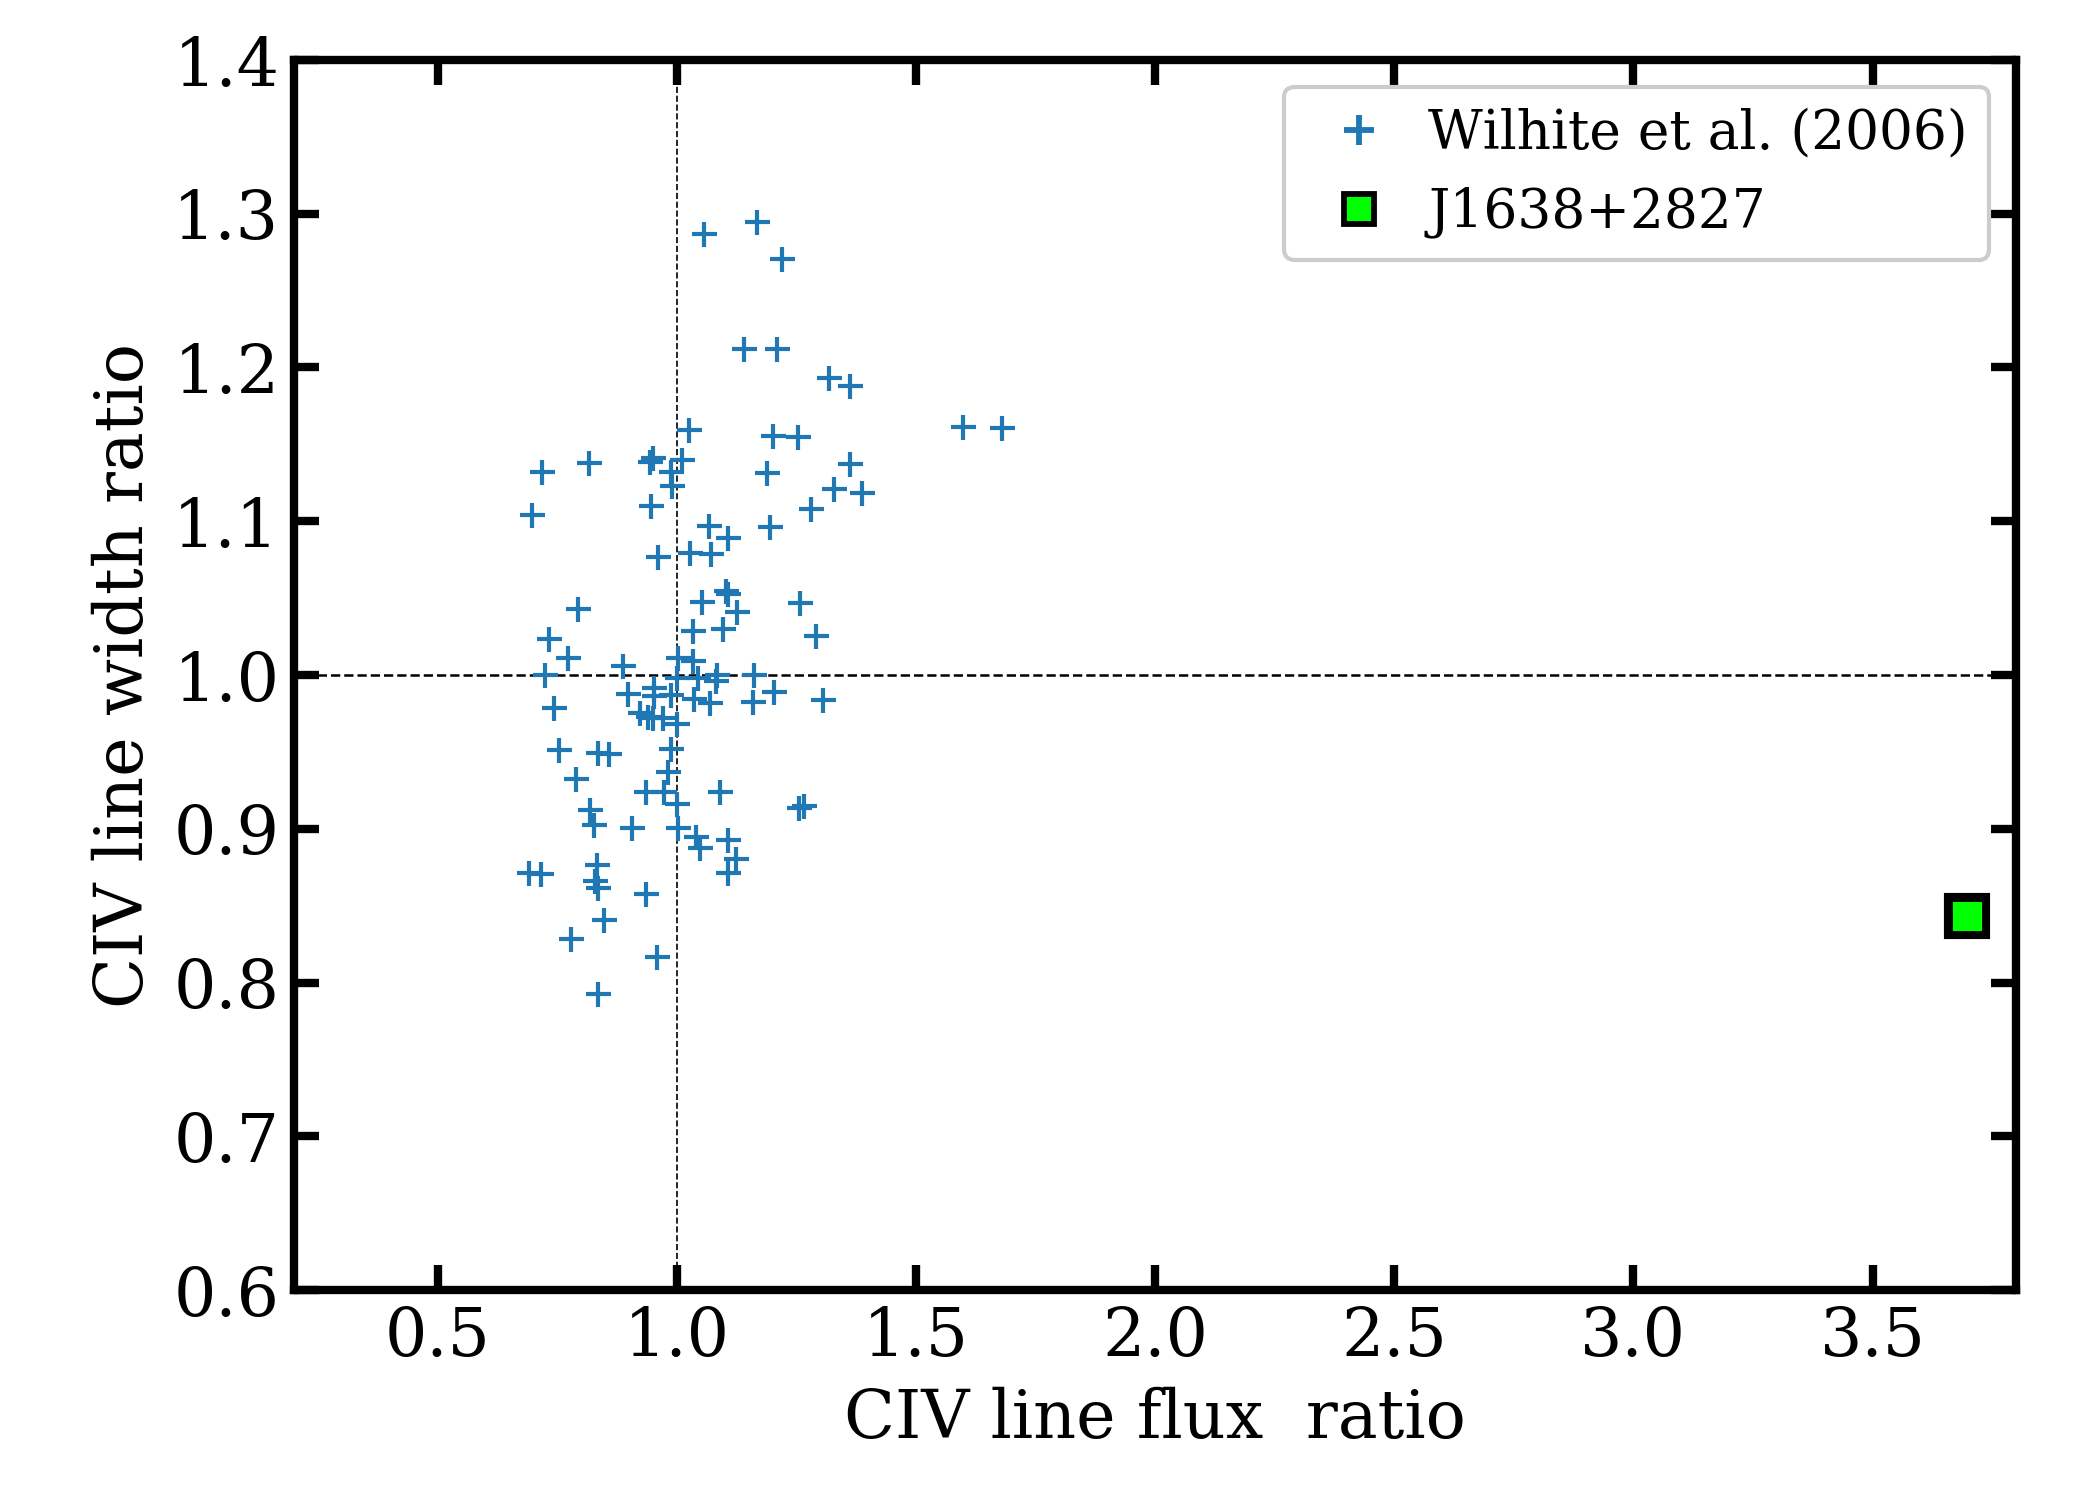
\includegraphics[width=8.7cm, trim=0.2cm 0.2cm 0.2cm 0.2cm, clip]
  {figures/Wilhite_2006_Fig2_redux_20190926.png}
   \vspace{-12pt}
  \caption[]{The Change in \civ\ line width vs. line flux change. 
We compare our object J1638+2827 with the sample 
from \citet{Wilhite2006} with a sample of 105 quasars observed at
multiple epochs by the SDSS. J1638+2827 is a substantial outlier 
in this parameter space.}
  \label{fig:Wilhite2006_comparison}
\end{figure}
From Figure~\ref{fig:Wilhite2006_comparison} there appears to be a
strong correlation between the change in the line flux and the change
in the line width.  Figure~\ref{fig:Wilhite2006_comparison} shows the
epoch-to-epoch flux ratio versus the ratio of line widths.

In the context of CLQs at lower-$z$...  
(Balmer CLQs vs. \civ CLQs...) 
Sociis natoque penatibus et
magnis dis parturient montes, nascetur ridiculus mus. Duis tempus,
lectus nec ultricies mollis, mi orci feugiat nulla, a bibendum velit
orci nec lacus. Duis a odio in nisi egestas dictum. Nullam vel quam
mauris, eget consectetur orci. Morbi ac mi sit amet neque consectetur
tempus ac eget est. Curabitur malesuada arcu sit amet metus dictum at
dapibus arcu accumsan. Fusce sollicitudin luctus rutrum.  

\begin{table*}
  \centering
  \begin{tabular}{l  lll  lll lll lll }
    \hline 
    \hline 
                    & \multicolumn{3}{l}{ {\bf J1205+3422}}          &  \multicolumn{6}{l}{{\bf J1638+2827}}                                                                                   &  \multicolumn{3}{l}{ {\bf J2228+2201}} \\
Emission      & \multicolumn{3}{l}{MJD 53498}                        & \multicolumn{3}{l}{MJD 54553}                        & \multicolumn{3}{l}{MJD 55832}                     &  \multicolumn{3}{l}{MJD 56189}     \\                 
line              & Line  $\sigma$ & Line  Flux &   Cont.  Flux   & Line  $\sigma$   & Line  Flux      & Cont.  Flux  & Line  $\sigma$ & Line  Flux  &   Cont. Flux  & Line  $\sigma$ & Line  Flux       &   Cont. Flux  \\    \hline                       
Ly$\alpha$  &   ---	        &	---      & ---                 &  1362	            &	510.5	    &	7.224          & 1769                 &  633.9	 &  5.376             & ---                   &  ---                & ---    \\
\nv	            & 1604	        & 1251        &  853.5             &  \; 854.6	    &	122.4   	    &	5.546          & 1012                 &  107.1	 &  4.645             &  5501	        &  611.3	          & -2.58  \\
$^{(a)}$\civ     & 2174	        & 1254	   &  661.6             &  1927	            &	462.6	    &	2.722         & 2287	               &  125.1	 &  1.256             &  2216	        & \; 48.67          &   0.49  \\
$^{(a)}$\heii    &  2174    	        & \;\; 33.2  &  620.3             &  1927    	            & \;\;\; 8.067  &	2.447         & 2287	               &  \; 10.7	 &  1.001             &  2216	        &  \;\;\; 0.35      &   0.39  \\
$^{(a)}$\ciii     & 2174	        & \;  449.4  &  523.6             &  1927    	            & \;\;\; 8.067  &	2.447         & 2287	               &  \; 10.7	 &  1.001             &  2216	        & \; 17.2             &  0.41  \\
$^{(a)}$\mgii   &  2174	        & \;	405.4  &  334.1             &  1927    	            & \;\;\; 8.067  &	2.447         & 2287	               &  \; 10.7	 &  1.001             &  2216	        & \; 33.6	           &  0.29  \\
    \hline 
   \hline   
  \end{tabular}
  \caption{Line Measurement Information from the SDSS DR12 Science Archive Server (SAS). 
    %dr12.sdss.org/spectrumDetail?plateid=2089\&mjd=53498\&fiber=427 
    Line $\sigma$ in units of   km s$^{-1}$; 
    Line flux          in units of  10$^{-17}$ erg/cm$^2$/s; 
    Continuum      in units of  10$^{-17}$ erg/cm$^2$/s/ \AA; 
    $^{(a)}$Emission lines of a common ``width group'', in this case,
    \civ1549, \heii1640, \ciii1909 and \mgii2800 are constrained to have
    the same intrinsic velocity width in the SDSS spectral line fitting
    procedure \citep{Bolton2012}.
  }
 \label{tab:SDSS_line_values}
\end{table*}


Lorem ipsum dolor sit amet, consectetur adipiscing elit. Aliquam porta
sodales est, vel cursus risus porta non. Vivamus vel pretium
velit. Sed fringilla suscipit felis, nec iaculis lacus convallis
ac. Fusce pellentesque condimentum dolor, quis vehicula tortor
hendrerit sed. Class aptent taciti sociosqu ad litora torquent per
conubia nostra, per inceptos himenaeos. Etiam interdum tristique diam
eu blandit. Donec in lacinia libero.

Sed elit massa, eleifend non sodales a, commodo ut felis. Sed id
pretium felis. Vestibulum et turpis vitae quam aliquam convallis. Sed
id ligula eu nulla ultrices tempus. Phasellus mattis erat quis metus
dignissim malesuada. Nulla tincidunt quam volutpat nibh facilisis
euismod. Cras vel auctor neque. Nam quis diam risus.



%%%%%%%%%%%%%%%%%%%%%%%%%%%%%%%%%%%%%%%%%%%%%%%%%%%%%%%%%%%%%%%%%%%%%%%%%%%%%
%%%%%%%%%%%%%%%%%%%%%%%%%%%%%%%%%%%%%%%%%%%%%%%%%%%%%%%%%%%%%%%%%%%%%%%%%%%%%
%%
%%   SECTION 4   SECTION 4   SECTION 4   SECTION 4   SECTION 4   SECTION 4  
%%   SECTION 4   SECTION 4   SECTION 4   SECTION 4   SECTION 4   SECTION 4  
%%   SECTION 4   SECTION 4   SECTION 4   SECTION 4   SECTION 4   SECTION 4  
%%
%%%%%%%%%%%%%%%%%%%%%%%%%%%%%%%%%%%%%%%%%%%%%%%%%%%%%%%%%%%%%%%%%%%%%%%%%%%%%
%%%%%%%%%%%%%%%%%%%%%%%%%%%%%%%%%%%%%%%%%%%%%%%%%%%%%%%%%%%%%%%%%%%%%%%%%%%%%
\begin{figure}
  \centering
  \includegraphics[width=8.7cm, trim=0.2cm 0.2cm 0.2cm 0.2cm, clip]
  {figures/CIV_CLQs_hexplot_20190925.png}
   \vspace{-12pt}
  \caption[]{The Rest Equivalent Width (REW) vs. Full Width Half Maximum (FWHM) 
of the \civ\ emission line in the BOSS DR12 quasar sample using the catalogue 
of \citet{Hamann2017}. Note the REW logarithmic scaling.}
  \label{fig:REWvsFWHM}
\end{figure}

\section{Discussion and Conclusions}
The variable properties of the rest-frame UV quasar emission lines
have been long studied, with the global (or ensemble) Baldwin Effect
(the anti-correlation between the EW of the emission line and the
underlying continuum luminosity of single-epoch observations of a
large number of AGN, first noted in \citet{Baldwin1977}. 
%%
More recently, the intrinsic Baldwin effect, the same anti-correlation but in an individual, variable AGN.
%
The variable properites of high-$z$ quasars, however, has been less 
well stuided. Reasons for this include more massive systems will tend to 
have longer timescales e.g. with $R_{\rm Sch}= 2GM /c^{2}$ and $t_{\rm dyn} =\sqrt{ R^{3}/GM}$
means   $t_{\rm dyn} \sim 6G^{3} M^{3} / GM c^{2} \sim 6G^{2} M^{2} / c^{2} $.

\noindent
{\bf Our Eddington ratios \\
Done 1\% \\
Coatman, Hewett say \civ\ masses are okay.\\
But what are these Eddington ratios? \\
Low state BHs vs. High-mass BHs... \\
Coatman et al?? Blue-shiftted \\
}

Nunc semper quam et leo interdum vulputate eu quis magna. Sed nec arcu
at orci egestas convallis. Aenean quam velit, aliquam vitae viverra
in, elementum vel elit. Nunc suscipit aliquet sapien a suscipit. Cras
nulla ipsum, posuere eu fringilla sit amet, dapibus ultricies
nulla. Nullam eu augue id purus mollis dignissim sed et
libero. Phasellus eget justo sed neque pellentesque egestas nec id
arcu. Donec facilisis pulvinar sapien et fringilla. Suspendisse
vestibulum rhoncus sapien id laoreet. Morbi et orci vitae tortor
imperdiet imperdiet. In hac habitasse platea dictumst. Vivamus vel
neque id mi ultrices tristique. Integer quam libero, ornare vel
gravida in, feugiat a ante. Nam dapibus, tellus vitae pellentesque
cursus, dui nisl egestas augue, non fermentum nisl est nec
nisi. Vestibulum nec mi justo, eget dapibus velit.

Etiam mollis viverra nisi eget aliquet. Aliquam erat volutpat. Vivamus
tristique, nisl eu malesuada semper, libero tortor convallis elit, a
scelerisque orci nisi lacinia turpis. In lacinia ultrices
volutpat. Proin ultrices luctus tellus, in placerat eros tincidunt
id. Ut varius iaculis quam in consequat. Nulla nec orci est, sit amet
pellentesque nisl. Mauris non cursus lectus. Praesent placerat leo vel
erat gravida lacinia. Donec vehicula consectetur lectus vitae
luctus. Praesent nisl justo, laoreet elementum facilisis vel,
tristique ac enim. Etiam vel quam ut quam eleifend
tincidunt. Suspendisse sit amet eros vel elit ullamcorper
laoreet. Etiam venenatis sodales turpis, nec lacinia ligula hendrerit
nec. Nam eu vulputate purus. Quisque facilisis congue metus, sed
imperdiet lorem rhoncus sit amet.

In this paper we have... 
\begin{itemize}
\item Pellentesque vel elit neque, in interdum lacus. Quisque sodales, nunc et luctus convallis, nisl dui luctus dui, at congue urna velit a; 
\item At sit amet sapien a risus dapibus sagittis. Cras sed ultricies erat. Donec id metus sed urna lacinia convallis vel sed enim. 
\item Nisi libero, ornare vel bibendum eu, sollicitudin sed leo. Cras tincidunt aliquet ultricies. Cras pretium velit leo, in malesuada. 
\item Duis sagittis ultricies interdum. Proin sit amet sem nec metus feugiat pharetra.
\end{itemize}

Aliquam ac metus nec odio tempus pharetra sed nec diam. Sed eget arcu
nulla. Etiam elementum ultrices ligula, at iaculis libero feugiat
bibendum. Suspendisse potenti. Nam pharetra adipiscing
euismod. Quisque imperdiet dignissim odio, sed volutpat justo
tincidunt eu. Nunc vehicula pharetra suscipit. Integer aliquet pretium
ipsum vel ultrices. Nam rutrum nibh ac quam pulvinar molestie.



\subsection*{Availability of Data and computer analysis codes} 
All materials, databases, data tables and code are fully available at: 
\href{https://github.com/d80b2t/VHzQ}{\tt https://github.com/d80b2t/}


\section*{Acknowledgements}
NPR acknowledges support from the STFC and the Ernest Rutherford Fellowship scheme. 
%% KESF \& BM are supported by NSF PAARE AST-1153335. 
%% KESF \& BM thank CalTech/JPL for support during sabbatical.  

\noindent
We thank:
\begin{list}{$\circ$}{}  
  \item Andy Lawrence, Mike Hawkins and David Homan for useful discussion. 
\end{list}

This paper heavily used \href{http://www.star.bris.ac.uk/~mbt/topcat/}{TOPCAT} (v4.4)
\citep[][]{Taylor2005, Taylor2011}.
%%
This research made use of \href{http://www.astropy.org}{\tt Astropy}, 
a community-developed core Python package for Astronomy 
\citep{AstropyCollaboration2013, AstropyCollaboration2018}.

Funding for SDSS-III has been provided by the Alfred P. Sloan
Foundation, the Participating Institutions, the National Science
Foundation, and the U.S. Department of Energy Office of Science. The
SDSS-III web site is
\href{http://www.sdss3.org/}{http://www.sdss3.org/}.
%%
SDSS-III is managed by the Astrophysical Research Consortium for the
Participating Institutions of the SDSS-III Collaboration including the
University of Arizona, the Brazilian Participation Group, Brookhaven
National Laboratory, Carnegie Mellon University, University of
Florida, the French Participation Group, the German Participation
Group, Harvard University, the Instituto de Astrofisica de Canarias,
the Michigan State/Notre Dame/JINA Participation Group, Johns Hopkins
University, Lawrence Berkeley National Laboratory, Max Planck
Institute for Astrophysics, Max Planck Institute for Extraterrestrial
Physics, New Mexico State University, New York University, Ohio State
University, Pennsylvania State University, University of Portsmouth,
Princeton University, the Spanish Participation Group, University of
Tokyo, University of Utah, Vanderbilt University, University of
Virginia, University of Washington, and Yale University.

This publication makes use of data products from the Wide-field
Infrared Survey Explorer, which is a joint project of the University
of California, Los Angeles, and the Jet Propulsion
Laboratory/California Institute of Technology, and NEOWISE, which is a
project of the Jet Propulsion Laboratory/California Institute of
Technology. WISE and NEOWISE are funded by the National Aeronautics
and Space Administration. No animals were harmed in the production of
this paper, but there was a large spider in NPRs apartment that
``vanished''.

\bibliographystyle{mnras}
\bibliography{tester_mnras}


% Don't change these lines
\bsp	% typesetting comment
\label{lastpage}
\end{document}


\end{document}